%!TEX root = ../paper.tex

\section{Introduction}
\label{sec:introduction}
% Proximity-based mobile apps
% Bluetooth Low Energy
% iBeacon protocol (see master project)
% Many applications (mainly in retailing)
% This paper... Smart Restaurant experience
% What are we trying to do
% Why? Improve service and bla bla bla (see abstract)
% Two mobile apps and a web app for waiters
% Present the rest of the document
Proximity-based apps are
context-aware apps that allow the user to interact
with the app if he is nearby some point of interest (POI).
Bluetooth is a wireless, short-range, communication technology.
Bluetooth Low Energy (BLE)\footnote{http://www.bluetooth.com/Pages/Bluetooth-Smart.aspx}
is an improvement of classic Bluetooth since it consumes
very low power, allowing it to be used by smaller devices.
And that is the main reason for this technology to start to
be used for proximity-based mobile apps,
BLE Beacons are devices, that use BLE, to broadcast a
Universally Unique Identifier (UUID).
These devices use the
iBeacon\footnote{http://developer.apple.com/ibeacon/}
protocol, which was created
by Apple\texttrademark. In this protocol the beacons
advertise the following sets of bytes, as it is shown in
figure \ref{fig:ibeacon}
(total 20 bytes, 160 bits):
\begin{description}
  \item[UUID] has 16 bytes and it is used to differentiate a
  large group of related beacons
  \item[Major] has 2 bytes and it is used to distinguish a smaller
  subset of beacons within the larger group
  \item[Minor] has 2 bytes and it is used to distinguish individual
  beacons within the smaller subset
\end{description}
A smartphone that
has BLE can get this signal with the mentioned bytes.
But, only smartphones
with Bluetooth, at least, version 4, have BLE.

\begin{figure}[!ht]
  \centering
    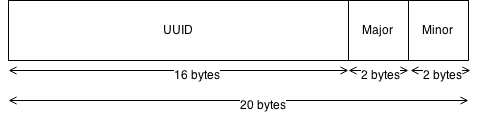
\includegraphics[width=0.9\textwidth]{figures/ibeacon}
    \caption{ibeacon protocol message structure}
    \label{fig:ibeacon}
\end{figure}

Next section, presents related work about existing applications using ibeacons.
Section \ref{sec:smart_restaurant_experience} shows the smart restaurant
experience and how customers, owners and waiters will take advantage of our
solution. Section \ref{sec:solution_architecture} describes the architecture
and its main components
of the solution being proposed here.
Section \ref{sec:conclusion_and_future_work} concludes the paper.
